\documentclass{article}
\usepackage{a4wide}


\usepackage{polski}
\usepackage[utf8x]{inputenc}
\usepackage{graphicx}
\usepackage{float}
\usepackage{hyperref}
\usepackage{listings}
\usepackage{mathtools}
\usepackage{amsmath}

\usepackage{color} %red, green, blue, yellow, cyan, magenta, black, white
\definecolor{mygreen}{RGB}{28,172,0} % color values Red, Green, Blue
\definecolor{taupe}{rgb}{0.28, 0.24, 0.2}
\definecolor{mylilas}{RGB}{0,110,0}


\author{Lev Sergeyev}
\title{SPC. Ćwiczenie 1. Sprawozdanie}

\date{2019.10}
\begin{document}

\maketitle

%\pagebreak

\section{Odpowiedź skokowa}
\par
Dany jest obiekt o transmitancji:
\begin{equation}
K(s)=\frac{1}{s^2+as+b} 
\end{equation}
\par
Dobierając parametry a i b otzrymano 4 pary biegunów. Dodatkowo przeprowadzona symulacja odpowiedzi układów na skok:

\begin{figure}
\scalebox{0.4}{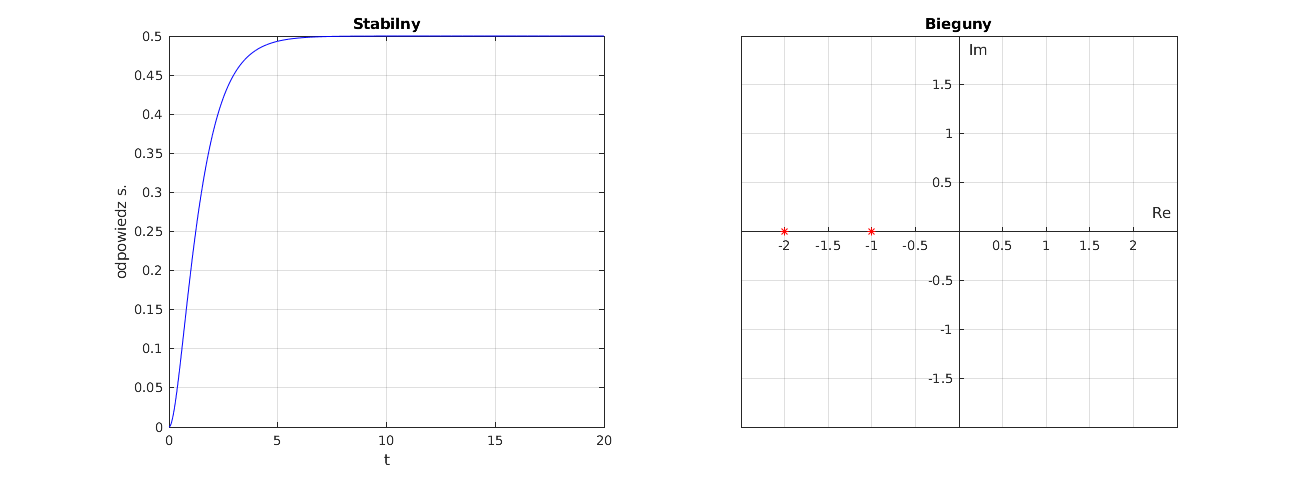
\includegraphics{skok/s1.png}}
\caption{Obiekt bez oscylacji, stabilny (a=3, b=2)}
\end{figure}

\begin{figure}
\scalebox{0.4}{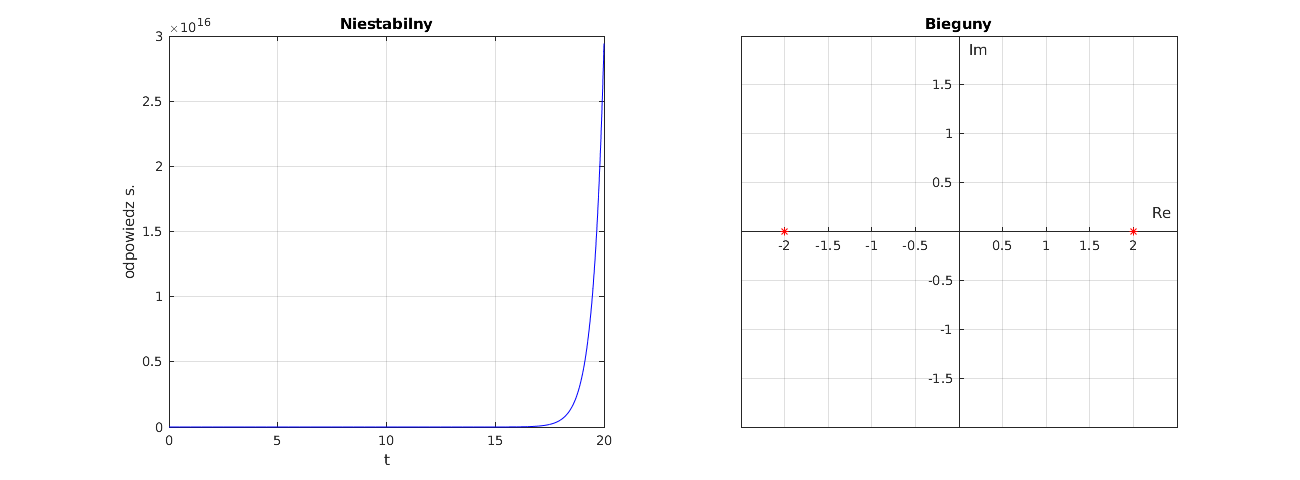
\includegraphics{skok/s3.png}}
\caption{Obiekt bez oscylacji, niestabilny (a=0, b=-4)}
\end{figure}

\begin{figure}
\scalebox{0.4}{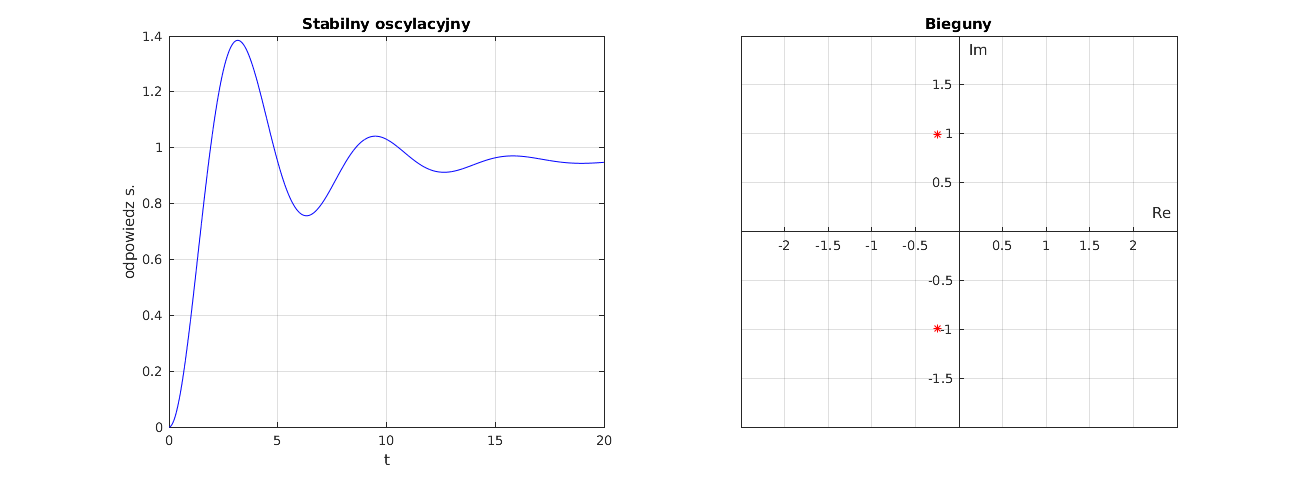
\includegraphics{skok/s4.png}}
\caption{Obiekt z oscylacją, stabilny (a=0.5, b=1.05)}
\end{figure}

\begin{figure}
\scalebox{0.4}{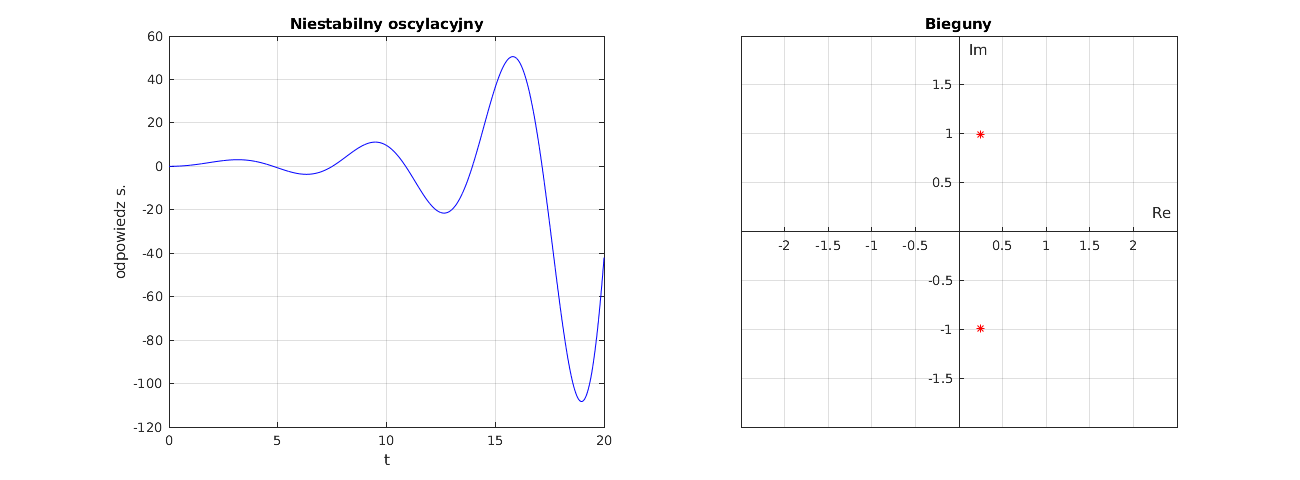
\includegraphics{skok/s6.png}}
\caption{Obiekt z oscylacją, niestabilny (a=-0.5, b=1.05)}
\end{figure}

\pagebreak

\section{Identyfikacja obiektu}
\par
Dana jest odpowiedź obiektu na wymuszenie skokowe \( ( \Delta = 1 )\) :


\begin{figure}[h]
\centering
\scalebox{0.25}{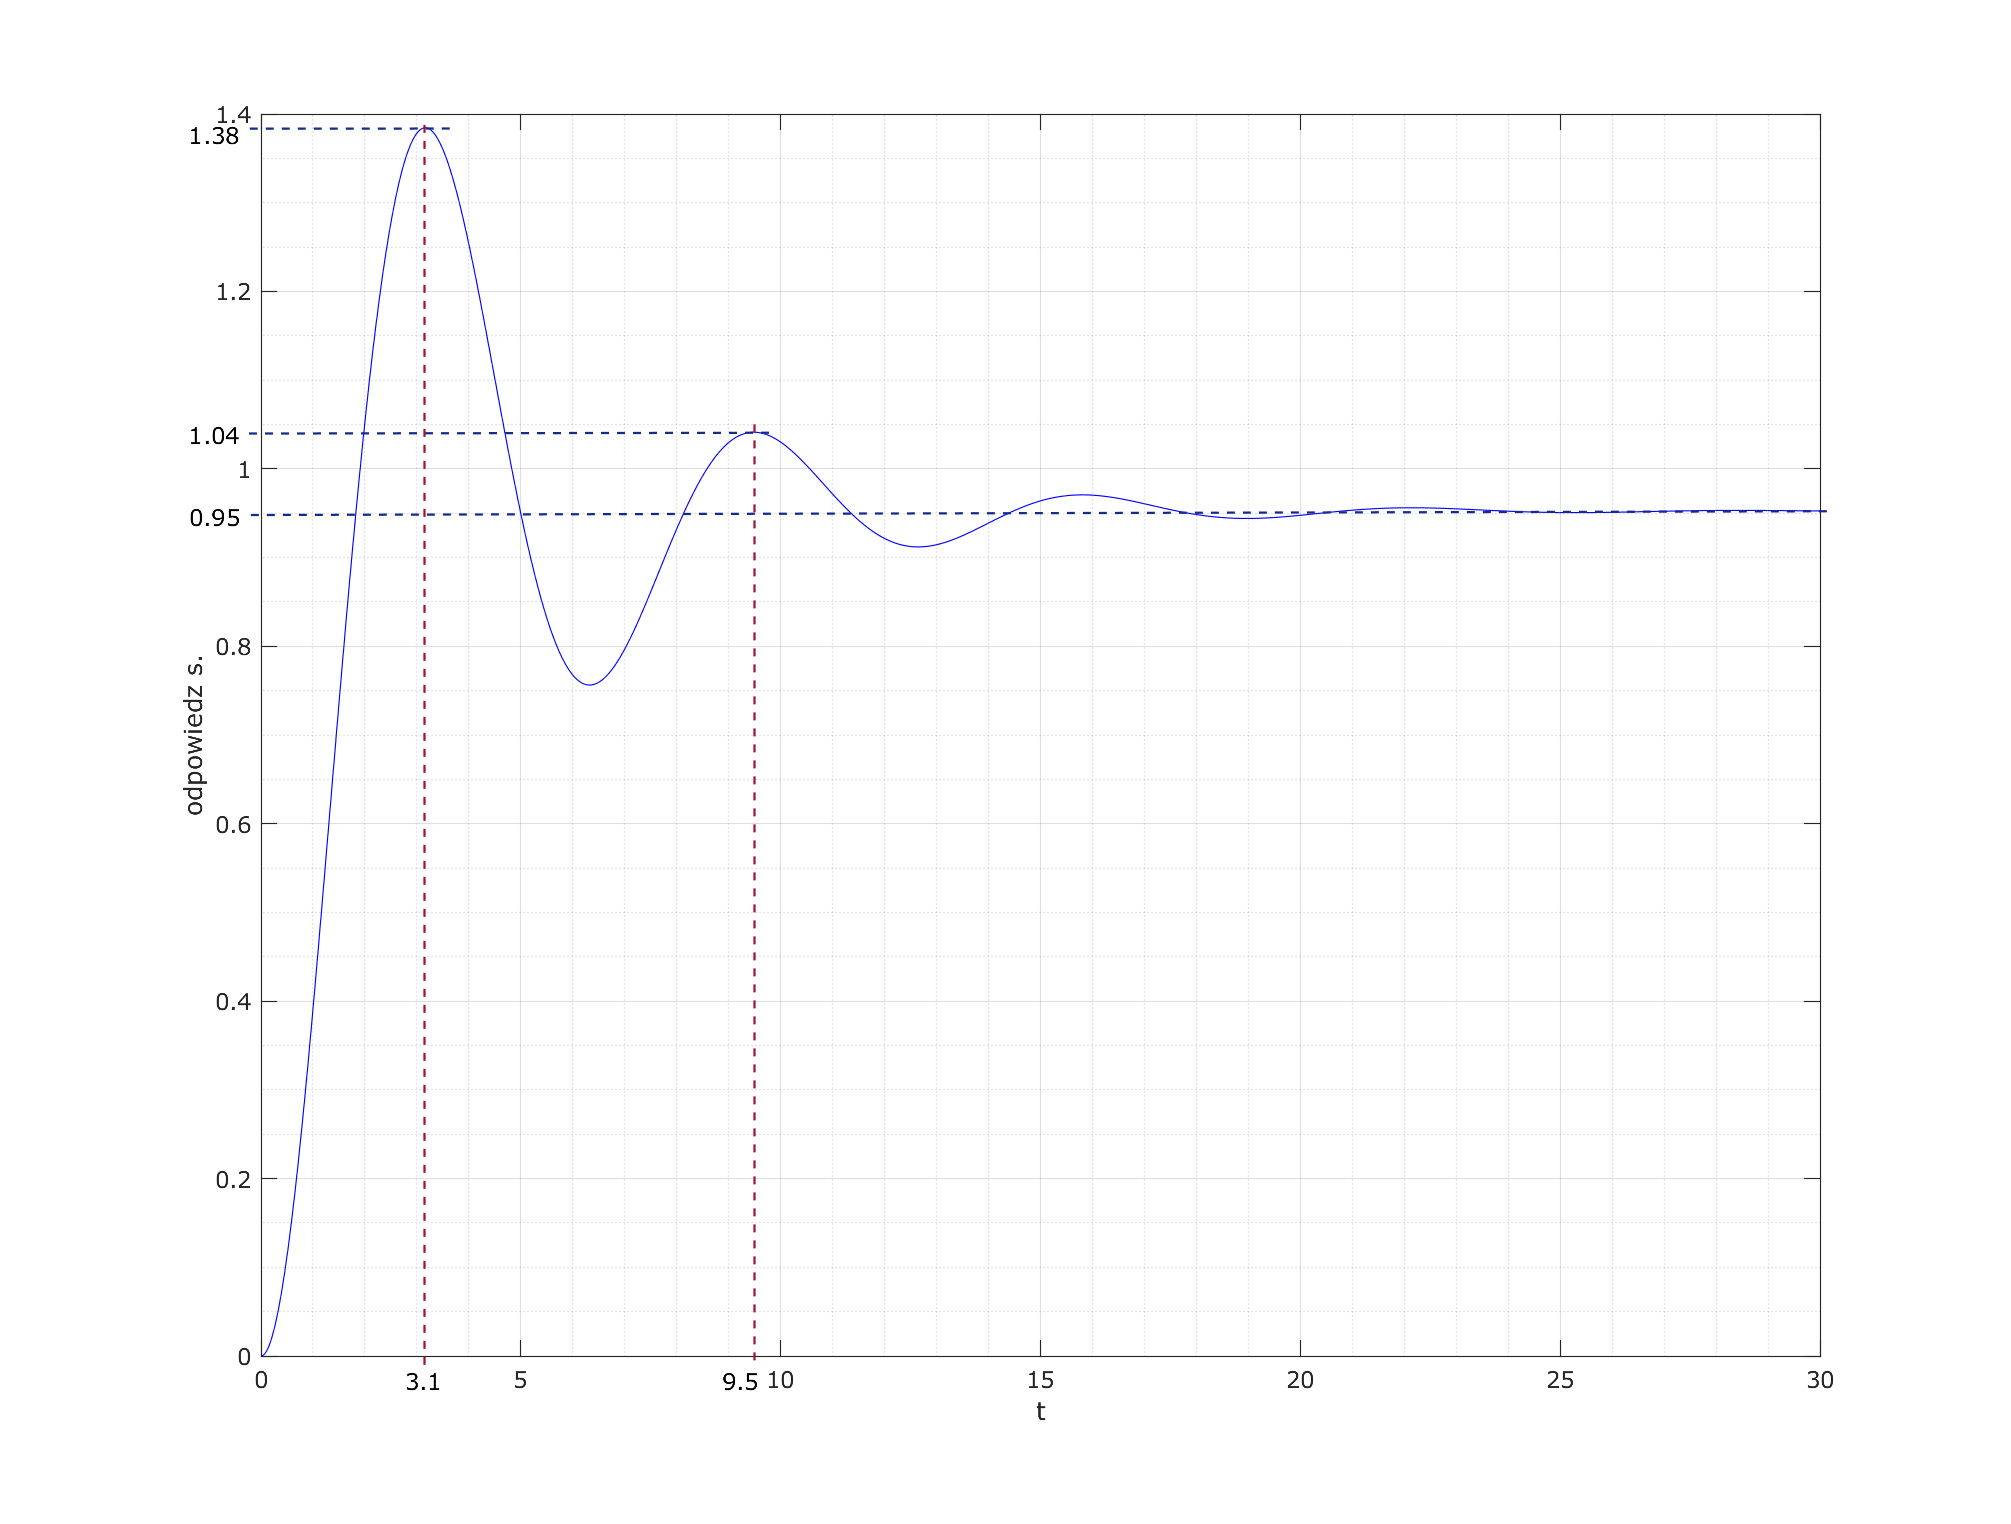
\includegraphics{identify/skok.png}}
\caption{Odpowedź badanego obiektu \( K(s)\)}
\end{figure}

Na podstawie tej odpowiedzi zidentyfikować obiekt.

Odpowiedź wskazuje na to, że badany obiekt składa się z członu oscylacyjnego i proporcyjnego, więc jego transmitancja ma postać:

\begin{equation}
K(s)=\frac{k \omega^{2}}{s^2+2 \xi \omega s + \omega^2} 
\end{equation}

Z wykresu można odczytać, że:

\begin{itemize}  
	\item \( k = 0.95 \)
	\item \( A_1 = 0.43 \)
	\item \( A_2 = 0.09 \)
	\item \( T_{A_2 - A_1} = 6.4 \)
\end{itemize}

Na podstawie odczytanych wartości obliczono \( \omega \) i \( \xi \):

\begin{equation}
\omega = \frac{ 2 \pi}{T} =  \frac{ 2 \pi}{6.4} = 0.98
\end{equation}

\begin{equation}
\xi = \frac{  \frac{A_1}{A_2} }{2 \pi} = 0.25
\end{equation}

Stąd otrzymano:

\begin{equation}
K(s)=\frac{k \omega^{2}}{s^2+2 \xi \omega + \omega^2}
= \frac{0.95*0.98^2}{s^2+2*0.25* 0.98*s + 0.98^2} = \frac{0.9124}{s^2 + 0.49s + 0.96}
\end{equation}


\section{Wnioski}

Dobierając bieguny transmitancji \(K(s)=\frac{1}{s^2+as+b} \) można otrzymać 6 typów układów: układy bez i z oscylacją, które można podzielić na stabilne, niestabilne i układy na granicy stabilności (w ćwiczeniu nie rozpatrzono przypadek układu na granicy stabilności). Więc w kryterium stabilności można brać mianownik układu.
\par
W drugiej części zadania zidentyfikowano układ na podstawie odpowiedzi układu na Rys. 3. Zastosowana graficzna metoda identyfikacji pozwoliła skutecznie wyznaczyć parametry układu takie, że \( a=0.49 \) i \( b=0.96 \), które są zbliżone do parametrów rzeczywistych \( (a=0.5, b=1.05) \).

\end{document}
